\documentclass{article}
\usepackage[utf8]{inputenc}
\usepackage[spanish]{babel}
\usepackage{listings}
\usepackage{graphicx}
\graphicspath{ {images/} }
\usepackage{cite}
\graphicspath{{Images/}}

\begin{document}

\begin{titlepage}
    \begin{center}
        \vspace*{0.2cm}
            
        \Huge
        \textbf{Proyecto de Investigación}
            
        \vspace{0.5cm}
        \LARGE
        Informática II
            
        \vspace{1cm}
            
        \textbf{Daniel Ovany Mesa López}
        
        \vfill
        
        \begin{figure}[htp]
            \centering
            
\includegraphics[width=8cm]{Images/Escudo_UdeA.png}
        \end{figure}
        
            
        \vspace{0.5cm}
            
        \Large
        Despartamento de Ingeniería Electrónica y Telecomunicaciones\\
        Universidad de Antioquia\\
        Medellín\\
        Septiembre de 2020
            
    \end{center}
\end{titlepage}


\newpage
\begin{center}
    \title{}
    \textbf{MEMORIA DE UN COMPUTADOR}    
\end{center}
\section*{Introducción:}
\begin{flushleft}
    Un sistema informático es un dispositivo electrónico que consta de dos componentes básicos: hardware y software, puede programarse para realizar diversas operaciones según las necesidades del usuario, necesita de un programa para realizar una operación específica. El sistema operativo asigna los recursos necesarios para ejecutar el programa en términos de espacio de memoria y tiempo de procesamiento de la CPU, esta inicia la ejecución del programa obteniendo la información del sistema de memoria.
    \begin{figure}[htp]
        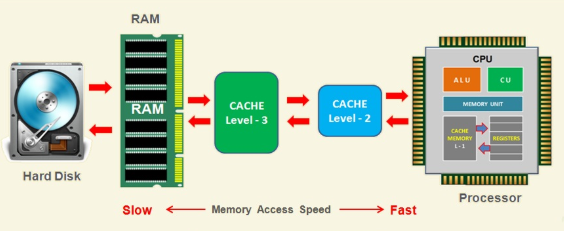
\includegraphics[width=14cm]{Images/Sistema de memoria.PNG}
        \caption{Jerarquía de la memoria del sistema de un computador}
        \label{hola:out}
    \end{figure}
    \begin{itemize}
        \item \textbf{Definición:} Una memoria es como un cerebro humano, se usa para almacenar información (Datos) o instrucciones (Programas de cómputo), el propósito de almacenamiento es guardar datos que el computador no esté utilizando.
        \item \textbf{Tipos de memorias:}\\
        -\textbf{Disco duro:} Es el dispositivo mécanico o de estado sólido en donde se puede almacenar la información e instrucciones a largo plazo, tienen la capacidad de leer o escribir la información que se le suministra.\\
        -\textbf{RAM:} Es un dispositivo electrónico que puede acceder a toda la información en cualquier momento, el procesamiento de esta es más rápido que el disco duro, una vez apagada la computadora la información se elimina lo cual su alamcenamiento es a corto plazo.\\
        -\textbf{Memoria flash:} Su funcionamiento es similar al de la RAM con la diferencia que son estables, incluso cuando no hay energía eléctrica alamcenan de forma segura la información, y cuentan con una capacidad de almacenamiento mucho meñor que el disco duro.\\
        -\textbf{ROM:} Los datos almacenados no pueden ser modificados ya que su acceso es solo para lectura, siempre mantiene la información independientemente si hay energía eléctrica o no, tiene una batería en el sistema y permite que se inicie la computadora cuando se requiera.\\
        \item \textbf{Gestión:} La memoria tiene como unidad básica de almacenamiento el dígito binario, cada uno de estos se almacenan en una celda de la memoria, la información e instrucciones contienen millones de bits que son procesados en la unidad de procesamiento central (CPU), cuando se hace un cambio en la información, el sistema operativo asigna un espacio dentro de la memoria RAM para dicho cambio, el tiempo requerido para hacerlo se conoce como latencia de la memoria. El intercambio de información entre la CPU y RAM es de baja latencia con respecto a la memoria caché interna que contiene la CPU, los cambios se pueden almacenar solo siempre y cuando la computadora esté encendida, entonces para que no se eliminen cuando se apague la computadora hay que transferirlos a un dispositivo de almacenamiento de largo plazo llamado disco duro.\\
        \item \textbf{Caracterización:} La estructura de la memoria en cualquier sistema informático se conforma por varios tipos de memoria que dependiendo del cambio que se realice con la información, sus componentes de fabricación y diseño físico controlarán el flujo de bits lo cual hará que una sea más rápida respecto a otra obteniendo una mayor eficiencia temporal y energética.
        \vfill
        %\bibliography{references}
        \begin{thebibliography}{X}
            \bibitem[1]{Aug} \textsc{Augusto Salazar},  \textsc{Nociones de la memoria del computador}, Medellín, 2020.
            \bibitem[2]{Dul} \textsc{Dulce María García Barrera}, \textsc{¿Cómo funciona la memoria de un computador?}, 2007. https://www.gestiopolis.com/como-funciona-memoria-computador/
            \bibitem[3]{Mar} \textsc{María Estela Raffino}, \textsc{Concepto de computadora}, Argentina, 2020. https://concepto.de/computadora/
        \end{thebibliography}
    \end{itemize}
\end{flushleft}


\end{document}
